\EnglishSourceFrame{GELFAND-P001405}{unlabelled}
Then
\begin{equation*}
(Y_I,Y_J)=\text{\EnglishUnclear{GELFAND-P001405}{pairing-value}{0 or C}}
\quad\text{for }J\ne I'.\tag{35}
\end{equation*}
(everything in the quotients)

\underline{Theorem:}

(36) $Z[x_1,x_2,x_3]$ is a free module [inserted above the line: over]
$\underline{\operatorname{Sym}}(x_1,x_2,x_3)$
with the Schubert polynomials as a basis.

Not all Schubert polynomials are determinants, so divided differences
$\partial_i$ are used instead.

\underline{Problem from I. M. G.} Generalise the theorem on characters: irreducible representations, characters
\EnglishUnclear{GELFAND-P001405}{characters-line-ending}{s-...- [unresolved source fragment]}
-Schubert functions.

\underline{Next time, Takhtajan will speak on quantum groups.}

\underline{\underline{Kapranov (Misha)}}

\underline{2-categories.}

This is an algebraic structure with objects of four types:
\begin{description}
\item[a)] objects $\bullet$
\item[b)] horizontal morphisms $\bullet\longrightarrow\bullet$
\item[c)] vertical morphisms $\uparrow$
\item[d)] squares
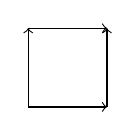
\begin{tikzpicture}[baseline=0.3cm]
\draw[->] (0,0)--(1,0);
\draw[->] (0,1)--(1,1);
\draw[->] (0,0)--(0,1);
\draw[->] (1,0)--(1,1);
\end{tikzpicture}
\end{description}

[In the right margin:]
Here $\begin{matrix}\longrightarrow\\\longrightarrow\end{matrix}$ are horizontal morphisms,
$\uparrow\ \uparrow$ vertical morphisms.
(Their beginnings and ends are 1-morphisms.)

One can compose:
\begin{description}
\item[1)] $\longrightarrow\ \longrightarrow$ two horizontal morphisms
\item[2)] $\begin{matrix}\uparrow\\\uparrow\end{matrix}$ two vertical morphisms
\item[3)] squares are multiplied in two ways
\end{description}
\begin{center}
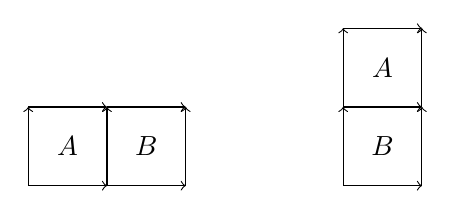
\begin{tikzpicture}
\draw[->] (0,0)--(1,0);
\draw[->] (1,0)--(2,0);
\draw[->] (0,1)--(1,1);
\draw[->] (1,1)--(2,1);
\draw[->] (0,0)--(0,1);
\draw[->] (1,0)--(1,1);
\draw[->] (2,0)--(2,1);
\node at (0.5,0.5) {$A$};
\node at (1.5,0.5) {$B$};
\draw[->] (4,0)--(5,0);
\draw[->] (4,1)--(5,1);
\draw[->] (4,2)--(5,2);
\draw[->] (4,0)--(4,1);
\draw[->] (4,1)--(4,2);
\draw[->] (5,0)--(5,1);
\draw[->] (5,1)--(5,2);
\node at (4.5,1.5) {$A$};
\node at (4.5,0.5) {$B$};
\end{tikzpicture}
\end{center}
(See Gabriel's book.)


\EnglishSourceFrame{GELFAND-P001406}{33}
\underline{The main nontrivial axiom}: two-dimensional associativity

(1)
\EnglishSourceFigure{GELFAND-P001406}{interchange-diagram}{On the left are two vertical rectangles: the first has $A$ above $B$, the second $C$ above a heavily retraced sign resembling $D$; the middle horizontal arrow in each points to the right. Between the rectangles is a composition circle, followed by an equals sign. On the right, the upper row contains $A$, $C$, the lower $B$ and a sign resembling $D$; between the rows is a narrow band with a circle. At the ends of the band are arrow-like and retraced strokes whose exact connections are unclear.}

\begin{center}
\begin{minipage}[t]{.46\linewidth}\vspace{0pt}\centering
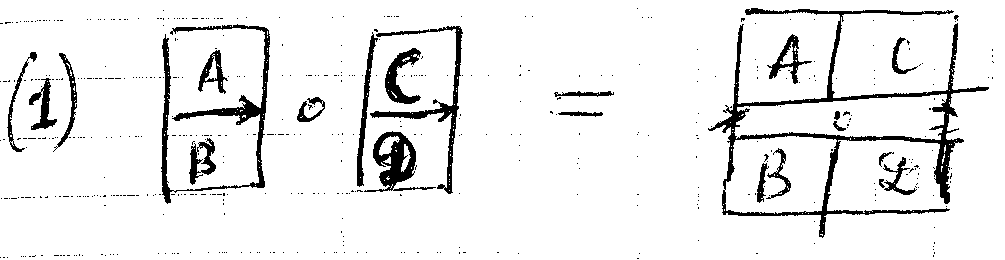
\includegraphics[width=\linewidth]{figures/gelfand-0153-p001406-interchange-original.png}\par\smallskip
{\footnotesize Original manuscript detail: \texttt{GELFAND-P001406}}
\end{minipage}\hfill
\begin{minipage}[t]{.50\linewidth}\vspace{0pt}\centering
{\footnotesize Partial visible-stroke recreation}\par\smallskip
\resizebox{\linewidth}{!}{% Visible-stroke transcription; D? and the retraced side connections remain unresolved.
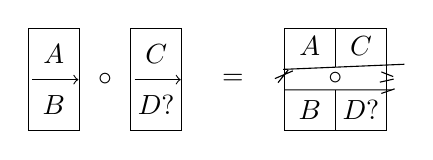
\begin{tikzpicture}[x=.65cm,y=.65cm]
\draw (0,0) rectangle (1,2); \draw[->] (.08,1)--(.98,1);
\node at (.5,1.5) {$A$};\node at (.5,.5) {$B$};
\node at (1.5,1) {$\circ$};
\draw (2,0) rectangle (3,2);\draw[->] (2.08,1)--(2.98,1);
\node at (2.5,1.5) {$C$};\node at (2.5,.5) {$D?$};
\node at (4,1) {$=$};
\draw (5,0)--(7,0)--(7,2)--(5,2)--cycle;
\draw (5,.8)--(7.1,.8) (4.98,1.2)--(7.35,1.3);
\draw (6,0)--(6,.8) (6,1.25)--(6,2);
\node at (5.5,1.65) {$A$};\node at (6.5,1.65) {$C$};
\node at (5.5,.4) {$B$};\node at (6.5,.4) {$D?$};
\node at (6,1.02) {$\circ$};
% Plain crossing strokes preserve uncertainty and do not declare arrows.
\draw (4.82,1.02)--(5.17,1.17) (4.88,.94)--(5.08,1.19);
\draw (6.9,1.15)--(7.13,1.06) (6.87,.95)--(7.14,1.01)
 (6.9,.73)--(7.16,.82);
\end{tikzpicture}
}
\end{minipage}
\end{center}
\noindent{\small\textit{The two D-like labels and retraced side strokes are unresolved. Plain side strokes do not declare arrow directions.}}


\underline{An example in which}
[crossed out: \EnglishUnclear{GELFAND-P001406}{example-cancel-left}{illegible}]
axiom
[crossed out: \EnglishUnclear{GELFAND-P001406}{example-cancel-right}{illegible}]
(1) \underline{does not hold}

\underline{Tensors:}
\begin{center}
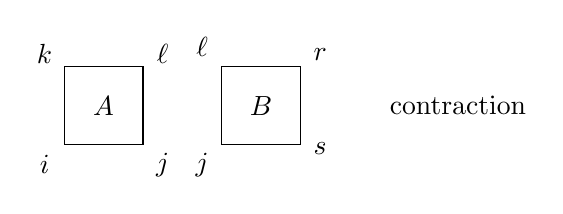
\begin{tikzpicture}
\draw (0,0)--(1,0)--(1,1)--(0,1)--cycle;
\node at (0.5,0.5) {$A$};
\node at (-0.25,1.15) {$k$};
\node at (1.25,1.15) {$\ell$};
\node at (-0.25,-0.25) {$i$};
\node at (1.25,-0.25) {$j$};
\draw (2,0)--(3,0)--(3,1)--(2,1)--cycle;
\node at (2.5,0.5) {$B$};
\node at (1.75,1.25) {$\ell$};
\node at (3.25,1.15) {$r$};
\node at (1.75,-0.25) {$j$};
\node at (3.25,-0.05) {$s$};
\node at (5,0.5) {contraction};
\end{tikzpicture}
\end{center}
\begin{equation*}
(AB)_{ik}^{rs}=\sum A_{ij}^{k\ell}B_{js}^{\ell r}
\end{equation*}
\EnglishUnclear{GELFAND-P001406}{tensor-indices}{The positions of the indices are retained from the manuscript.}

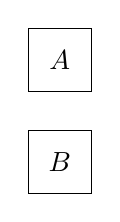
\begin{tikzpicture}
\draw (0,1.3)--(0.8,1.3)--(0.8,2.1)--(0,2.1)--cycle;
\node at (0.4,1.7) {$A$};
\draw (0,0)--(0.8,0)--(0.8,0.8)--(0,0.8)--cycle;
\node at (0.4,0.4) {$B$};
\end{tikzpicture}

Axiom (1) will not hold.

\underline{Another definition} (M. Kontsevich) (a competing one)

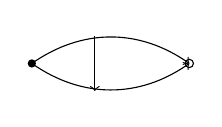
\begin{tikzpicture}[baseline=0cm]
\fill (0,0) circle (1.5pt);
\draw (2,0) circle (1.5pt);
\draw[->] (0,0) to[bend left=35] (2,0);
\draw[->] (0,0) to[bend right=35] (2,0);
\draw[->] (0.8,0.35)--(0.8,-0.35);
\end{tikzpicture}
Morphisms between morphisms with the same endpoints.

\underline{Example:} $Cat$ (the category of categories; there is a morphism
of functors)

This is a special case of the preceding definition (contract the vertical arrows).

\underline{I. M. G.}

\EnglishSourceFigure{GELFAND-P001406}{boundary-diagram}{Inside the square is written $\Delta u=0$. Along the upper and lower sides, horizontal arrows point to the right; beside the left side, two interior vertical arrows point upwards. On the left are the labels $u$ and $\frac{\partial u}{\partial n}$; above that label is another unclear notation.}

\begin{center}
\begin{minipage}[t]{.46\linewidth}\vspace{0pt}\centering
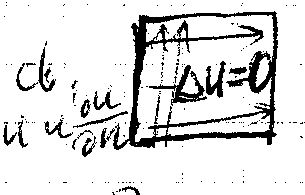
\includegraphics[width=\linewidth]{figures/gelfand-0153-p001406-boundary-original.png}\par\smallskip
{\footnotesize Original manuscript detail: \texttt{GELFAND-P001406}}
\end{minipage}\hfill
\begin{minipage}[t]{.50\linewidth}\vspace{0pt}\centering
{\footnotesize Partial visible-stroke recreation}\par\smallskip
\resizebox{\linewidth}{!}{\begin{tikzpicture}[x=1.2cm,y=1.2cm]
\draw (0,0) rectangle (1.1,1);
\draw[->] (.05,.83)--(1.04,.83);\draw[->] (.03,.13)--(1.06,.19);
\draw[->] (.15,.1)--(.19,.95);\draw[->] (.29,.13)--(.36,.96);
\node at (.69,.55) {$\Delta u=0$};
\node[left] at (-.05,.6) {$[?]$};
\node[left] at (-.06,.05) {$u,\ \dfrac{\partial u}{\partial n}$};
\end{tikzpicture}
}
\end{minipage}
\end{center}
\noindent{\small\textit{The upper left notation remains [?] after 3×, 5× and 10× inspection. The visible u and normal derivative are typed; no boundary condition is supplied.}}

Boundary conditions

A request to Keldysh--Chentsov--Gelfand

\underline{K.} Higher fundamental groups.
$X_0\subset X_1\subset X$ is a topological space.

Objects are points $x\in X_0$.

Morphisms
$\bigl(\underset{\text{interval}}{I},\partial I\bigr)\longrightarrow(X_1,X_0)$;
homotopic ones $(\mathrm{mod}\ \partial I)$ are considered equivalent.

Bimorphisms
$(I^2,\partial I^2)\longrightarrow(X,X_1)$
\qquad $(\mathrm{mod}\ \text{\underline{homotopy}})$


\EnglishSourceFrame{GELFAND-P001407}{44}
\underline{\underline{23/XI-87.}} \qquad \underline{Gelfand seminar.}

\underline{Beilinson} (continued)

\underline{Derived categories.}

(1) \underline{Lemma:}
\begin{equation*}
\begin{tikzcd}[column sep=small,row sep=small]
X^\bullet && Y^\bullet\\
& Z^\bullet \arrow[ul,"{\text{quasi-isomorphism}}"] \arrow[ur] &
\end{tikzcd}
\quad\Rightarrow\quad\exists\quad
\begin{tikzcd}[column sep=small,row sep=small]
& Z'^\bullet &\\
X^\bullet \arrow[ur,"{\text{quasi-isomorphism}}"] && Y^\bullet \arrow[ul]
\end{tikzcd}
\end{equation*}

The lemma is proved using the mapping-cone construction.

\underline{Reminder:}

$\mathcal{A}$ is an abelian category.
\begin{equation*}
\begin{array}{ccccc}
C(\mathcal{A}) & \longrightarrow & K(\mathcal{A}) & \longrightarrow & D(\mathcal{A})\\
\text{complexes} && \substack{\text{homotopy}\\\text{category}\\\text{of complexes}} &&
\substack{\text{derived}\\\text{category}}
\end{array}
\end{equation*}
[On the right:] (the objects are complexes throughout).

$f:X^\bullet\to Y^\bullet$ is homotopic to $0$ if
$\exists g^i:X^i\to Y^{i-1}$,
\begin{equation*}
f^i=dg^i+g^{i+1}d
\end{equation*}

$D(\mathcal{A})$ is $K(\mathcal{A})$ with the
\underline{quasi-isomorphisms} inverted
(morphisms inducing isomorphisms of cohomology).

A morphism from $X^\bullet$ to $Y^\bullet$ is a diagram in $K(\mathcal{A})$:
\begin{equation*}
\begin{tikzcd}[column sep=small,row sep=small]
X^\bullet && Y^\bullet\\
& Z^\bullet \arrow[ul,"\sim"] \arrow[ur] &
\end{tikzcd}
\tag{2}
\end{equation*}
(The left arrow is a quasi-isomorphism.)

More precisely, an equivalence class of such diagrams: diagram (2) is equivalent to
the diagram obtained using any quasi-isomorphism
$\chi:Z'^\bullet\to Z^\bullet$:
\begin{equation*}
\begin{tikzcd}[column sep=small,row sep=small]
X^\bullet && Y^\bullet\\
& Z^\bullet \arrow[ul,"\varphi"',"\sim"] \arrow[ur,"\psi"] &\\
& Z'^\bullet \arrow[u,"\chi"',"\sim"] &
\end{tikzcd}
\qquad
\begin{tikzcd}[column sep=small,row sep=small]
X^\bullet && Y^\bullet\\
& Z' \arrow[ul,"{\varphi\circ\chi}"',"\sim"] \arrow[ur,"{\psi\circ\chi}"'] &
\end{tikzcd}
\tag{3}
\end{equation*}

(Extend this relation to the smallest equivalence relation containing it.)

The cone of a morphism and exact triangles were defined
[crossed out: \EnglishUnclear{GELFAND-P001407}{last-line-cancellation}{illegible}]
also [source final word: ``eshchyo''].


\EnglishSourceFrame{GELFAND-P001408}{unlabelled}
\underline{I. Zakharevich}
[crossed out: \EnglishUnclear{GELFAND-P001408}{cancelled-title}{illegible}]
\underline{Improvisation \EnglishUnclear{GELFAND-P001408}{title-preposition}{about / with} chaos.}

\underline{Examples}

$1^{\circ}$. Apparently there is a morphism from one example to the other.
\begin{equation*}
M=(\mathbb{Z}/2\mathbb{Z})^{\mathbb{Z}}
\qquad\text{(a sequence infinite in both directions)}
\end{equation*}
$T\colon M\to M$. On $M$ is the standard topology (a Cantor set).
\begin{equation*}
a_i\to a_{i-1}\qquad\text{(the shift transformation; the Bernoulli transformation)}
\end{equation*}
Consider the iterates: $T^N$.

There is a measure on $M$. The baker transformation coincides with this
[inserted above the line: (up to measure $0$)]
[crossed out after ``this'' and in the line below:
\EnglishUnclear{GELFAND-P001408}{baker-cancellations}{illegible}].

\begin{center}
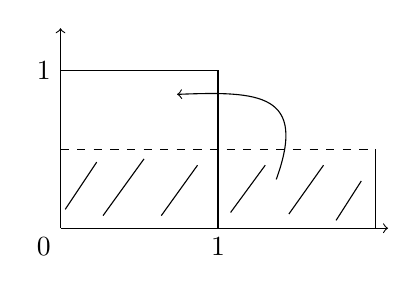
\begin{tikzpicture}[x=2cm,y=2cm]
\draw[->] (0,0) -- (2.08,0);
\draw[->] (0,0) -- (0,1.27);
\draw (0,1) -- (1,1) -- (1,0);
\draw (2,0) -- (2,0.5);
\draw[dashed] (0,0.5) -- (2,0.5);
\draw (0.03,0.12) -- (0.23,0.42);
\draw (0.27,0.08) -- (0.53,0.44);
\draw (0.64,0.08) -- (0.87,0.4);
\draw (1.08,0.1) -- (1.3,0.4);
\draw (1.45,0.09) -- (1.67,0.4);
\draw (1.75,0.05) -- (1.91,0.3);
\draw[->] (1.37,0.31) .. controls (1.57,0.86) and (1.26,0.87) .. (0.74,0.85);
\node[below left] at (0,0) {$0$};
\node[left] at (0,1) {$1$};
\node[below] at (1,0) {$1$};
\end{tikzpicture}
\end{center}

\EnglishSourceFigure{GELFAND-P001408}{baker-sequence}{Three drawings from left to right: a square with a closed rounded curve and a horizontal dashed line; a square with two elongated bends entering from opposite sides; a square with several nearly horizontal strips and short loop-shaped bends at the edges. The third drawing has a distinguishable left-pointing arrow on its lower long line; the directions of small strokes in the first and third drawings are not entirely clear.}

\begin{center}
\begin{minipage}[t]{.46\linewidth}\vspace{0pt}\centering
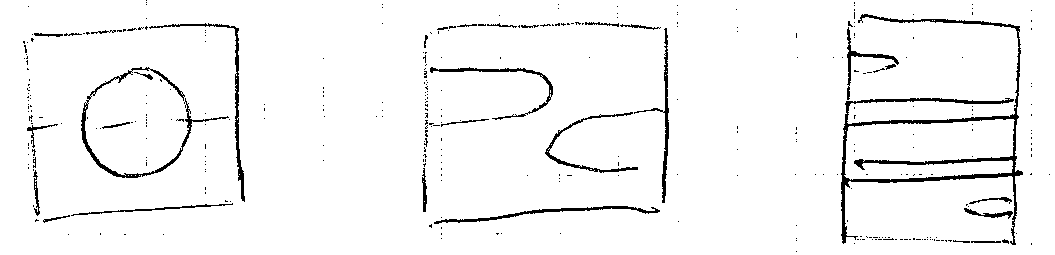
\includegraphics[width=\linewidth]{figures/gelfand-0153-p001408-baker-sequence-original.png}\par\smallskip
{\footnotesize Original manuscript detail: \texttt{GELFAND-P001408}}
\end{minipage}\hfill
\begin{minipage}[t]{.50\linewidth}\vspace{0pt}\centering
{\footnotesize Partial visible-stroke recreation}\par\smallskip
\resizebox{\linewidth}{!}{% Only the clear leftward long arrow is interpreted as a direction.
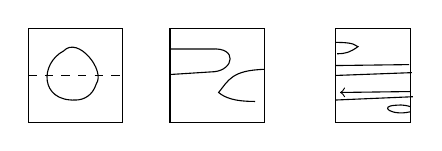
\begin{tikzpicture}[x=.6cm,y=.6cm]
\draw (0,0) rectangle (2,2);\draw[dashed] (0,1)--(2,1);
\draw (1,.48) .. controls (.25,.45) and (.24,1.25) .. (.75,1.52)
 .. controls (1.05,1.84) and (1.64,1.11) .. (1.44,.82)
 .. controls (1.36,.57) and (1.17,.48) .. (1,.48);
\draw (3,0) rectangle (5,2);
\draw (3,1.56)--(3.88,1.56) .. controls (4.44,1.6) and (4.35,1.12) .. (3.94,1.08)--(3,1.02);
\draw (5,1.13) .. controls (4.31,1.11) and (4.24,.9) .. (4.03,.64)
 .. controls (4.16,.53) and (4.36,.45) .. (4.8,.45);
\draw (6.5,0) rectangle (8.1,2);
\draw (6.5,1.7) .. controls (6.93,1.7) and (6.9,1.64) .. (6.98,1.61)
 .. controls (6.81,1.49) and (6.72,1.46) .. (6.54,1.46);
\draw (6.5,1.21)--(8.06,1.23) (6.5,1.0)--(8.12,1.06);
\draw[->] (8.1,.66)--(6.6,.64);\draw (6.5,.48)--(8.14,.55);
\draw (8.08,.23) .. controls (7.7,.14) and (7.4,.35) .. (7.78,.37)
 .. controls (7.93,.39) and (8.07,.35) .. (8.08,.34);
\end{tikzpicture}
}
\end{minipage}
\end{center}
\noindent{\small\textit{Visible bends are preserved. Only the clear long left-pointing arrow is assigned a direction; small endpoint strokes remain uninterpreted.}}

And so on.

\underline{Correspondence}: write the coordinates of a point of the square in binary
and take $1$ digit to the left, another to the right.

In what sense is this chaos?

Consider $T^k x$, $k\leq 0$; suppose this is known (to within $1$ mm).
\begin{equation*}
T^k x,\qquad k>0
\end{equation*}
In finite time, all this information will be lost.

$2^{\circ}$. \underline{Hyperbolic transformation}:
geodesic flows on \EnglishUnclear{GELFAND-P001408}{manifold-abbreviation}{mn-ziyakh / mn-iyakh [unexpanded source abbreviations]} of negative curvature.

\EnglishSourceFigure{GELFAND-P001408}{hyperbolic-surface}{A closed contour with two expanded parts and a constriction between them. Inside, on the left and right, arcs resemble indications of two handles of a surface; the middle contains a short slanting segment with marked endpoints and a branching arrow upwards to the right. Small directions and the exact connections of the interior arcs require comparison with the original.}

\begin{center}
\begin{minipage}[t]{.46\linewidth}\vspace{0pt}\centering
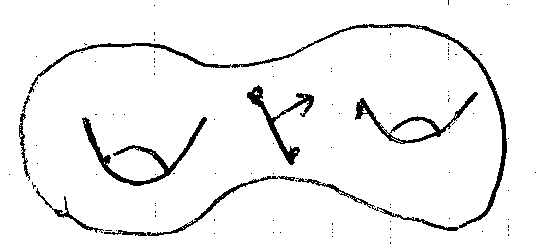
\includegraphics[width=\linewidth]{figures/gelfand-0153-p001408-hyperbolic-surface-original.png}\par\smallskip
{\footnotesize Original manuscript detail: \texttt{GELFAND-P001408}}
\end{minipage}\hfill
\begin{minipage}[t]{.50\linewidth}\vspace{0pt}\centering
{\footnotesize Partial visible-stroke recreation}\par\smallskip
\resizebox{\linewidth}{!}{% The drawn contour and interior arcs are reproduced without a genus assertion.
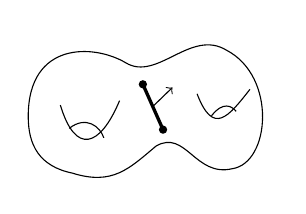
\begin{tikzpicture}[x=.8cm,y=.8cm]
\draw (0,1) .. controls (0,2.2) and (1.05,2.15) .. (1.55,1.85)
 .. controls (2.05,1.55) and (2.58,2.4) .. (3.15,2.05)
 .. controls (3.95,1.63) and (3.84,.26) .. (3.24,.17)
 .. controls (2.65,.03) and (2.5,.8) .. (2.03,.53)
 .. controls (1.6,.17) and (1.34,-.1) .. (.7,.1)
 .. controls (.17,.21) and (0,.55) .. (0,1);
\draw (.51,1.18) .. controls (.75,.38) and (1.14,.51) .. (1.45,1.25);
\draw (.65,.81) .. controls (.92,1.02) and (1.14,.84) .. (1.2,.66);
\draw (2.68,1.36) .. controls (2.94,.68) and (3.18,1.0) .. (3.52,1.43);
\draw (2.91,1.01) .. controls (3.09,1.24) and (3.23,1.17) .. (3.3,1.08);
\draw[very thick] (1.82,1.51)--(2.14,.79);
\fill (1.82,1.51) circle (1.5pt);\fill (2.14,.79) circle (1.5pt);
\draw[->] (1.97,1.15)--(2.29,1.46);
\end{tikzpicture}
}
\end{minipage}
\end{center}
\noindent{\small\textit{The outer contour, interior arcs, marked segment and branch arrow are recreated. No topology or metric is inferred from the sketch.}}



\EnglishSourceFrame{GELFAND-P001409}{45}
\underline{G. Margulis.}
\underline{Iterates of maps of the complex plane.}

Consider the transformation $z\to P(z)$, where $P$ is a polynomial

(more generally, a rational function).

$\operatorname{deg}P=1$
[crossed out: \EnglishUnclear{GELFAND-P001409}{degree-one-cancellation}{illegible}]
is an uninteresting case.

$(1)\quad z\mapsto az+b$

\underline{Iterates}:
\begin{equation*}
z_{i+1}=P(z_i)
\end{equation*}
$|a|>1\Rightarrow$ one fixed point;

\EnglishUnclear{GELFAND-P001409}{unit-modulus-claim}{$|a|=1\Rightarrow$ everything splits into invariant circles, on which there is a rotation.}

\begin{center}
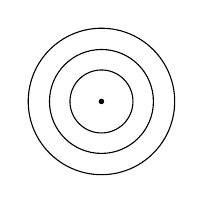
\begin{tikzpicture}
\draw (0,0) circle (0.4);
\draw (0,0) circle (0.66);
\draw (0,0) circle (0.93);
\fill (0,0) circle (0.035);
\end{tikzpicture}
\end{center}

\underline{I. M. G.}: 1) The question of when a transformation of the circle is diffeomorphic to a rotation
is nontrivial: Denjoy, Arnold, Herman.

2) What is a representation of a discrete infinite group?

There is no satisfactory answer.

Von Neumann theory is not aesthetically pleasing.

Chaos arises on the circle.

\underline{Conjecture}: if one works with sets of intermediate Hausdorff
dimension, some classical theory will be restored!!

\underline{Question for schoolchildren}: cover the $n$th rational number by an interval
of length $\varepsilon/2^n$. Give an example of a number which will not be covered.

\underline{Problem}: find the Hausdorff dimension of the Cantor perfect set.

\tikz\node[draw,circle,inner sep=2pt] {!};
\underline{Problem}. \underline{Construct a representation theory of discrete groups on functions on}
\underline{sets of intermediate Hausdorff dimension.}

To begin with, look at physics---string theory and so on.

\underline{G. M.}:
$z\to z^2$
\qquad $|z|=1$ maps to itself.

\begin{center}
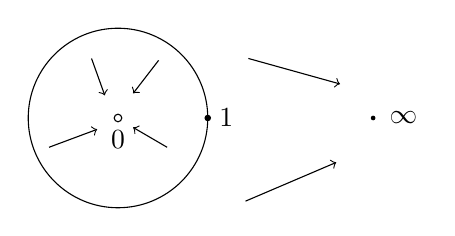
\begin{tikzpicture}[x=1.2cm,y=1.2cm]
\draw (0,0) circle (0.95);
\draw (0,0) circle (0.04);
\node[below] at (0,-0.03) {$0$};
\fill (0.95,0) circle (0.035);
\node[right] at (0.97,0) {$1$};
\draw[->] (-0.28,0.63) -- (-0.14,0.24);
\draw[->] (0.43,0.61) -- (0.16,0.26);
\draw[->] (0.52,-0.31) -- (0.16,-0.1);
\draw[->] (-0.73,-0.31) -- (-0.22,-0.12);
\draw[->] (1.38,0.63) -- (2.35,0.36);
\draw[->] (1.35,-0.88) -- (2.31,-0.47);
\fill (2.7,0) circle (0.025);
\node[right] at (2.77,0) {$\infty$};
\end{tikzpicture}
\end{center}
On the circle, this is an analogue of the (one-sided)
baker transformation.


\EnglishSourceFrame{GELFAND-P001410}{unlabelled}
\begin{equation*}
f_n=\underbrace{f\circ f\circ\cdots\circ f}_{n\ \text{times}}
\end{equation*}
\underline{Definition}

$U$ is a [crossed out: set; inserted above the line: neighbourhood]
of normality if $\left.f_n\right|_U$ is a compact set

(a normal family of analytic functions).

[On a separate short line, crossed out:
\EnglishUnclear{GELFAND-P001410}{isolated-cancellation}{illegible}.]

The set of normality [inserted above the line: $X$] consists of points $x$ for which
$\exists$ a neighbourhood $U$---[crossed out:
\EnglishUnclear{GELFAND-P001410}{normality-cancellation}{illegible}]
a neighbourhood of normality.

[Beneath ``set of normality'': (it is open).]

The complement of the set of normality is the \underline{Julia set}.

(It is closed.)

The set of normality may be empty.

\begin{equation*}
X=X_1\cup\cdots\cup X_n\cup\cdots
\end{equation*}
(connected components)

of the set of normality

[crossed out beneath this caption:
\EnglishUnclear{GELFAND-P001410}{components-cancellation}{illegible}]

\begin{equation*}
\begin{aligned}
f\colon (\text{connected components})&\to(\text{connected components})\\
X_i&\mapsto X_{j(i)}
\end{aligned}
\end{equation*}
\underline{Sullivan} proved that in the resulting

[crossed out: \EnglishUnclear{GELFAND-P001410}{sullivan-cancellation}{illegible}]
transformation of a discrete set (countable or finite),

a) every orbit stabilises,

b) the set of fixed points is finite.

\underline{Idea of the proof}. Suppose that there is an infinite orbit.

\begin{center}
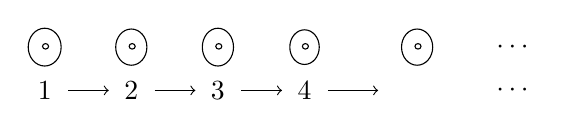
\begin{tikzpicture}[x=1.1cm,y=1cm]
\draw (0,0) ellipse (0.19 and 0.24);
\draw (0.01,0.01) circle (0.035);
\draw (1,0) ellipse (0.18 and 0.23);
\draw (1.01,0.01) circle (0.035);
\draw (2,0) ellipse (0.18 and 0.24);
\draw (2.01,0.01) circle (0.035);
\draw (3,0) ellipse (0.17 and 0.22);
\draw (3.01,0.01) circle (0.035);
\draw (4.3,0) ellipse (0.18 and 0.23);
\draw (4.31,0.01) circle (0.035);
\node at (5.4,0) {$\cdots$};
\node at (0,-0.55) {$1$};
\node at (1,-0.55) {$2$};
\node at (2,-0.55) {$3$};
\node at (3,-0.55) {$4$};
\draw[->] (0.27,-0.55) -- (0.74,-0.55);
\draw[->] (1.27,-0.55) -- (1.74,-0.55);
\draw[->] (2.27,-0.55) -- (2.74,-0.55);
\draw[->] (3.27,-0.55) -- (3.85,-0.55);
\node at (5.4,-0.55) {$\cdots$};
\end{tikzpicture}
\end{center}

Make a change of conformal
[crossed out: \EnglishUnclear{GELFAND-P001410}{structure-cancellation}{transf. [source abbreviation] / illegible}]
structure, so that the transformation remains
conformal.

\underline{Problem}:

\EnglishSourceFigure{GELFAND-P001410}{circle-packing}{Inside a square are four large rounded contours, two in the upper and two in the lower row; smaller closed curves occupy the gaps and border. On the right, a horizontal arrow points towards the square, with the caption ``inscribe''. Exact tangencies and which contours contain small boundary arcs are not entirely distinguishable.}

\def\GelfandPackingCaption{inscribe}
\begin{center}
\begin{minipage}[t]{.46\linewidth}\vspace{0pt}\centering
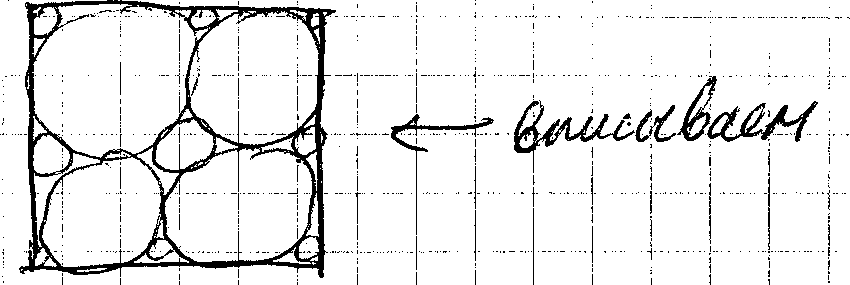
\includegraphics[width=\linewidth]{figures/gelfand-0153-p001410-circle-packing-original-r2.png}\par\smallskip
{\footnotesize Original manuscript detail: \texttt{GELFAND-P001410}}
\end{minipage}\hfill
\begin{minipage}[t]{.50\linewidth}\vspace{0pt}\centering
{\footnotesize Partial visible-stroke recreation}\par\smallskip
\resizebox{\linewidth}{!}{% Hand-drawn contours; these coordinates do not specify exact tangencies or radii.
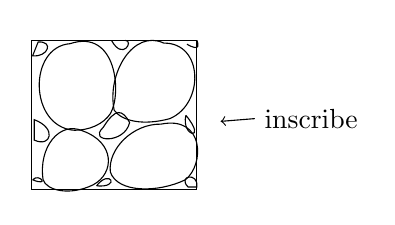
\begin{tikzpicture}[x=.7cm,y=.7cm]
\draw (0,0) rectangle (3,2.7);
\draw (.75,1.07) .. controls (-.05,1.16) and (-.06,2.58) .. (.7,2.64)
 .. controls (1.55,2.92) and (1.64,1.72) .. (1.43,1.37)
 .. controls (1.31,1.19) and (1.06,1.06) .. (.75,1.07);
\draw (1.5,1.43) .. controls (1.36,2.1) and (1.85,2.91) .. (2.4,2.65)
 .. controls (3.12,2.66) and (3.14,1.55) .. (2.51,1.28)
 .. controls (2.03,1.15) and (1.65,1.23) .. (1.5,1.43);
\draw (.21,.17) .. controls (.12,.76) and (.51,1.24) .. (.92,1.06)
 .. controls (1.52,.85) and (1.51,.29) .. (1.12,.08)
 .. controls (.69,-.13) and (.27,-.02) .. (.21,.17);
\draw (1.43,.31) .. controls (1.38,.73) and (1.84,1.19) .. (2.35,1.18)
 .. controls (3.14,1.34) and (3.14,.44) .. (2.79,.17)
 .. controls (2.29,-.07) and (1.56,-.07) .. (1.43,.31);
\draw (.02,2.42) .. controls (.3,2.39) and (.41,2.69) .. (.12,2.67)--cycle;
\draw (1.45,2.7) .. controls (1.66,2.32) and (1.86,2.7) .. (1.7,2.7);
\draw (2.82,2.63) .. controls (3.08,2.48) and (3.02,2.65) .. (3,2.7);
\draw (.05,.89) .. controls (.36,.75) and (.46,1.11) .. (.05,1.26)--cycle;
\draw (1.3,1.12) .. controls (1.01,.85) and (1.69,.81) .. (1.78,1.21)
 .. controls (1.65,1.44) and (1.53,1.49) .. (1.3,1.12);
\draw (2.8,1.34) .. controls (3.2,.86) and (2.71,.94) .. (2.8,1.34);
\draw (.02,.17) .. controls (.34,.04) and (.14,.3) .. (.02,.17);
\draw (1.18,.06) .. controls (1.42,.38) and (1.63,.02) .. (1.18,.06);
\draw (2.84,.04) .. controls (2.64,.24) and (3.03,.32) .. (3,.04)--cycle;
\draw[->] (4.05,1.28)--(3.43,1.23);
\node[right] at (4.05,1.28) {\GelfandPackingCaption};
\end{tikzpicture}
}
\end{minipage}
\end{center}
\noindent{\small\textit{The visible contours are recreated approximately. Exact tangencies, circle sizes and the inclusion of small boundary arcs remain unresolved; the reconstruction specifies no quantitative packing.}}


1) Prove that the remainder has measure $0$.

2) Prove that the remainder has Hausdorff dimension $<2$.


\EnglishSourceFrame{GELFAND-P001411}{46}
\underline{\underline{I. M. Gelfand}}. \underline{Matroids.}

In a $K$-dimensional space, consider $n$ vectors;
enumerate them and compile a list of which are linearly dependent and which are not.
Specifying this list gives a \underline{matroid}.

What conditions must this list satisfy?

\underline{Example}:
[Crossed out: \EnglishUnclear{GELFAND-P001411}{example-cancelled}{illegible}.]

\begin{center}
\begin{minipage}[t]{.46\linewidth}\vspace{0pt}\centering
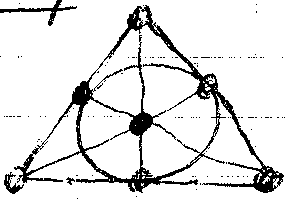
\includegraphics[width=\linewidth]{figures/gelfand-0153-p001411-fano-points-original.png}\par\smallskip
{\footnotesize Original manuscript detail: \texttt{GELFAND-P001411}}
\end{minipage}\hfill
\begin{minipage}[t]{.50\linewidth}\vspace{0pt}\centering
{\footnotesize Partial visible-stroke recreation}\par\smallskip
\resizebox{\linewidth}{!}{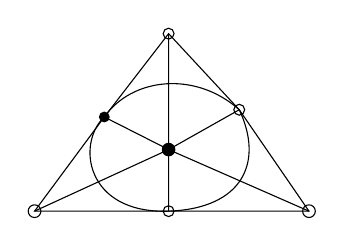
\begin{tikzpicture}[scale=1.15]
\coordinate (a) at (0,1.96);
\coordinate (b) at (-1.48,0);
\coordinate (c) at (1.55,0);
\coordinate (d) at (-0.71,1.04);
\coordinate (e) at (0.78,1.12);
\coordinate (f) at (0,0);
\coordinate (g) at (0,0.68);
\draw (a)--(d)--(b)--(f)--(c)--(e)--cycle;
\draw (a)--(g)--(f) (b)--(g)--(e) (d)--(g)--(c);
\draw (d) .. controls (-0.40,1.48) and (0.30,1.55) .. (e)
 .. controls (1.05,0.55) and (0.83,0.03) .. (f)
 .. controls (-0.92,-0.03) and (-1.02,0.75) .. (d);
\draw (a) circle (0.06) (b) circle (0.07) (c) circle (0.07)
 (e) circle (0.06) (f) circle (0.06);
\fill (d) circle (0.06) (g) circle (0.075);
\end{tikzpicture}
}
\end{minipage}
\end{center}
\noindent{\small\textit{The seven points retain the two filled and five outlined markings of the diplomatic drawing. No vector labels are added.}}


If three points lie on one line, the vectors
are linearly dependent.

The whole space is three-dimensional (there are no four linearly independent vectors).

(1) \underline{Problem}: 1) Prove that such vectors do not exist over $\mathbb{R}$ and $\mathbb{C}$!

2) Such vectors do exist over $\mathbb{Z}/2\mathbb{Z}$.

(All nonzero vectors in $(\mathbb{Z}/2\mathbb{Z})^3$!)

\underline{General} (\underline{unsolved problem}): which matroids are realised
a) over $\mathbb{R}$,
b) over $\mathbb{C}$.?

\underline{Solved problem}: which matroids are realised over $\forall$ fields?

\underline{In Rota's book} \EnglishUnclear{GELFAND-P001411}{book-after-rota}{e.. [source Cyrillic sign]}
[On the right: see \EnglishUnclear{GELFAND-P001411}{book-overwritten-noun}{book? [uncertain source ending]} \underline{Aigner} (?)]
there are fifteen different equivalent definitions of a matroid.

(2) \underline{Axioms}.

Certain subsets are distinguished and \underline{called bases}.

$B_1,B_2$ are two bases.

$y\in B_2,\ y\notin B_1\ \Rightarrow\ \exists x\in B_1;$
$(B_1\setminus x)\cup y$
[Crossed out: \EnglishUnclear{GELFAND-P001411}{basis-exchange-cancelled}{illegible}],
$(B_2\setminus y)\cup x$ are
\newline
bases.

\underline{Exercise in linear algebra}: verify this for a set of vectors in a vector space.

(3) \underline{Bimatroid}: consider a matrix; it defines two matroids, from its columns
and rows:

$S$ and $T$.

Another notion: list all minors $\ne0$.

Bimatroid: a family of subsets with the same number of elements.

(4) [Crossed out: \EnglishUnclear{GELFAND-P001411}{problem-four-cancelled}{illegible}.]
\underline{Problem}: state axioms for a bimatroid.


\EnglishSourceFrame{GELFAND-P001412}{unlabelled}
(5) \underline{Problem}: how is the bimatroid notion from
[Crossed out: \EnglishUnclear{GELFAND-P001412}{top-cancelled}{illegible}]
Gelfand--Serganova (UMN)
related to \EnglishUnclear{GELFAND-P001412}{knuth-name}{Kunt [source candidate: «Кунтом»]}?

\underline{Problem}: prove that

\begin{equation*}
\text{(6)}\quad
[x_1,\ldots,x_d][y_1,\ldots,y_d]
=\sum(-1)^{d-i}[y_1,x_2,\ldots,x_d]
[y_1,\ldots,y_{i-1},x_i,y_{i+1},\ldots,y_d]
\end{equation*}
\EnglishUnclear{GELFAND-P001412}{determinant-formula-source}{The indices $y_1$, $x_i$ and sign $(-1)^{d-i}$ are as in the manuscript.}

$[x_1,\ldots,x_d]$ is the determinant formed from the vectors.

(7) \underline{Remark}: if $[x_1,\ldots,x_d]$, $[y_1,\ldots,y_d]$ are bases, the right side has
a nonzero summand; this gives the exchange axiom
\EnglishUnclear{GELFAND-P001412}{basis-axiom-reference}{(3)}.

(\EnglishUnclear{GELFAND-P001412}{overwritten-eight}{8})
\underline{Problem} (tedious). Hilbert's chain of syzygies:
\begin{equation*}
(\text{ring})\longmapsto
\underset{\text{--- determinants}}{(\text{generators})}
\longmapsto (\text{relations between generators})
\end{equation*}

(9) (\underline{Assertion}: (6) gives all relations between the generators.)

(10) a) Write the whole chain!

b) Discretise the whole chain (write combinatorial relations).

(11) \underline{Problem}. A bimatroid---a list of minors $\longrightarrow$
[Crossed out: \EnglishUnclear{GELFAND-P001412}{problem-eleven-cancelled}{illegible}]
two matroids
(rows and columns).

A bimatroid is constructed from two matroids.

\EnglishSourceFigure{GELFAND-P001412}{basis-grid}{A grid of four vertical and four horizontal lines; braces on the left and below carry labels ``baz...'' [source beginnings]; an arrow on the right points leftwards towards the grid.}

\def\GelfandBasisLabel{baz... [?]}
\begin{center}
\begin{minipage}[t]{.46\linewidth}\vspace{0pt}\centering
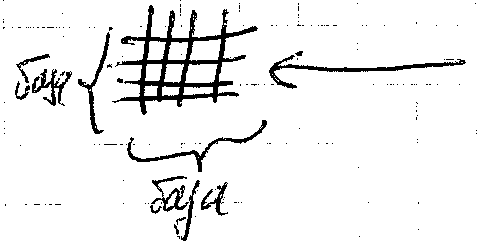
\includegraphics[width=\linewidth]{figures/gelfand-0153-p001412-basis-grid-original.png}\par\smallskip
{\footnotesize Original manuscript detail: \texttt{GELFAND-P001412}}
\end{minipage}\hfill
\begin{minipage}[t]{.50\linewidth}\vspace{0pt}\centering
{\footnotesize Partial visible-stroke recreation}\par\smallskip
\resizebox{\linewidth}{!}{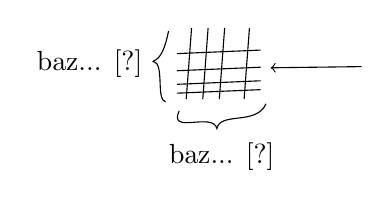
\begin{tikzpicture}[x=.75cm,y=.75cm]
\foreach \x in {0,.28,.56,.98}{\draw (\x,-.1)--(\x+.09,1.1);}
\foreach \y in {0,.15,.38,.67}{\draw (-.16,\y)--(1.26,\y+.06);}
\draw (-.3,1.05) .. controls (-.35,.8) and (-.42,.59) .. (-.56,.54)
 .. controls (-.36,.5) and (-.52,-.1) .. (-.35,-.15);
\draw (-.12,-.3) .. controls (-.31,-.71) and (.45,-.31) .. (.52,-.6)
 .. controls (.57,-.31) and (1.19,-.55) .. (1.35,-.18);
\node[left] at (-.58,.5) {\GelfandBasisLabel};
\node[below] at (.6,-.68) {\GelfandBasisLabel};
\draw[->] (2.97,.45)--(1.43,.43);
\end{tikzpicture}
}
\end{minipage}
\end{center}
\noindent{\small\textit{Both brace labels retain only the source beginning baz...; their endings remain unresolved after 3×, 5× and 10× inspection. Row and column basis terminology does not settle their glyphs.}}


by the definition of \EnglishUnclear{GELFAND-P001412}{basis-construction-word}{baza? [unresolved source form]}.

But this is not necessarily so.

A bimatroid contains more information.

What is the additional information in a bimatroid?

This is an important cohomological notion.

\underline{Remark}. Algebraic topology is a small island in familiar
combinatorial techniques.


\EnglishSourceFrame{GELFAND-P001413}{unlabelled}
\underline{\underline{30/XI-87.}}\qquad \underline{Gelfand seminar.}

\underline{I. M. Gelfand.} Problem: find the characters of the symmetric group.

(Following Frobenius.)

\underline{On the paper by} \underline{Kerov}: ``\underline{Realisation of representations of the Hecke algebra}, etc.''

Hint: these are characters of the symmetric group.

The Hecke algebra is the algebra with generators $\{e_k\}$
[above the line: $k=1,\ldots,N-1$] and relations
\begin{equation*}
\text{(1)}\quad
\left\{\begin{aligned}
e_k e_{k+1}e_k-\tau e_k&=e_{k+1}e_k e_{k+1}-\tau e_{k+1}\\
e_{k+j}e_k&=e_k e_{k+j},\quad j\geq 2;\\
e_k^2&=e_k
\end{aligned}\right.
\end{equation*}
Other generators
\begin{equation*}
\text{(2)}\quad \sigma_k=(q+1)e_k-1,\qquad \tau=\frac{q}{(q+1)^2}
\end{equation*}
This algebra is denoted by $H_N(q)$.

\underline{Exercise}: write the relations for $\sigma_k$.

(3) For $q=1$ (or $\tau=\frac14$), one obtains the group algebra of the symmetric group.

(4) \underline{Problem}: $\dim H_N(q)=N!$

[In the left margin: a circled ``!''.]
In the paper by \EnglishUnclear{GELFAND-P001413}{citation-name}{Tipper / Dipper} and James,

Proc. London Math. Soc.\qquad 1986, v. 52, p. 20--52

Recommended!!

it is proved that the representation theory of $H_N(q)$ is analogous to the theory of modular
representations of the symmetric group.

This works even in the complex case (see the paper by Bernsh.--Gelf.--Gelf.
on Verma modules).

Here it is assumed that $q\ne\sqrt[m]{1}$.

\underline{Construction of representations.}

A Young diagram\quad $\lambda=(\lambda_1,\lambda_2,\ldots,\lambda_k)$

\begin{center}
(5)\qquad
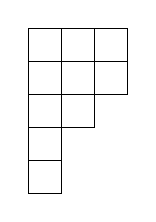
\begin{tikzpicture}[x=0.42cm,y=0.42cm]
\draw (0,0)--(3,0)--(3,-2)--(2,-2)--(2,-3)--(1,-3)--(1,-5)--(0,-5)--cycle;
\draw (1,0)--(1,-5);
\draw (2,0)--(2,-3);
\draw (0,-1)--(3,-1);
\draw (0,-2)--(3,-2);
\draw (0,-3)--(2,-3);
\draw (0,-4)--(1,-4);
\end{tikzpicture}
\qquad
$\begin{gathered}\sum\lambda_j=|\lambda|\\[8pt]\lambda_{i+1}\leq\lambda_i\end{gathered}$
\end{center}

($\lambda_i$ is the number of cells in the $i$th column.)

This corresponds to a conjugacy class of elements.


\EnglishSourceFrame{GELFAND-P001414}{52}
A Young tableau:
\begin{equation*}
\text{(6)}\quad t=\{\lambda^{(k)}\}_{k=1}^{N}
\quad\text{--- a family of diagrams in which}
\end{equation*}
\begin{equation*}
|\lambda^{(k)}|=k.
\end{equation*}

The usual definition (a different one): the tableau is filled with the numbers $1,2,\ldots,|\lambda|$, with
\begin{equation*}
\begin{matrix}\rightarrow\\\downarrow\end{matrix}
\quad\text{increase in these directions}
\end{equation*}

\begin{center}
\begin{minipage}[t]{.46\linewidth}\vspace{0pt}\centering
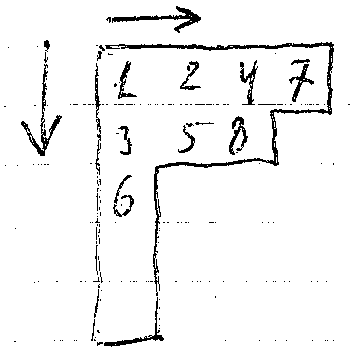
\includegraphics[width=\linewidth]{figures/gelfand-0153-p001414-young-tableau-original.png}\par\smallskip
{\footnotesize Original manuscript detail: \texttt{GELFAND-P001414}}
\end{minipage}\hfill
\begin{minipage}[t]{.50\linewidth}\vspace{0pt}\centering
{\footnotesize Partial visible-stroke recreation}\par\smallskip
\resizebox{\linewidth}{!}{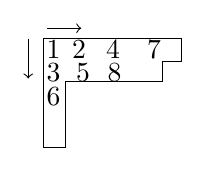
\begin{tikzpicture}[x=0.44cm,y=0.44cm]
\draw (0,0)--(4,0)--(4,-0.65)--(3.45,-0.65)--(3.45,-1.25)--(0.65,-1.25)--(0.65,-3.15)--(0,-3.15)--cycle;
\node at (0.30,-0.33) {$1$};
\node at (1.04,-0.33) {$2$};
\node at (2.02,-0.33) {$4$};
\node at (3.20,-0.33) {$7$};
\node at (0.30,-0.97) {$3$};
\node at (1.15,-0.97) {$5$};
\node at (2.06,-0.97) {$8$};
\node at (0.30,-1.66) {$6$};
\draw[->] (0.12,0.30)--(1.10,0.30);
\draw[->] (-0.43,0.0)--(-0.43,-1.15);
\end{tikzpicture}
}
\end{minipage}
\end{center}
\noindent{\small\textit{The irregular outline and the eight visible numbers are retained. The blank long leg is not filled and no internal cell grid is supplied.}}


In (6), they must increase.

\begin{center}
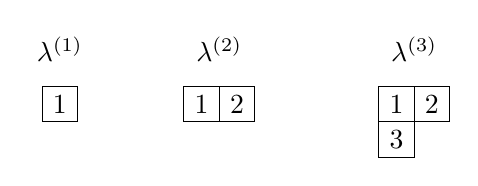
\begin{tikzpicture}[x=0.45cm,y=0.45cm]
\node at (0.5,1.05) {$\lambda^{(1)}$};
\draw (0,0) rectangle (1,-1);
\node at (0.5,-0.5) {$1$};
\node at (5,1.05) {$\lambda^{(2)}$};
\draw (4,0) rectangle (6,-1);
\draw (5,0)--(5,-1);
\node at (4.5,-0.5) {$1$};
\node at (5.5,-0.5) {$2$};
\node at (10.5,1.05) {$\lambda^{(3)}$};
\draw (9.5,0)--(11.5,0)--(11.5,-1)--(10.5,-1)--(10.5,-2)--(9.5,-2)--cycle;
\draw (10.5,0)--(10.5,-1);
\draw (9.5,-1)--(10.5,-1);
\node at (10,-0.5) {$1$};
\node at (11,-0.5) {$2$};
\node at (10,-1.5) {$3$};
\end{tikzpicture}
\end{center}

\begin{equation*}
\text{(7)}\quad r_k(t)=(i_{k+1}-j_{k+1})-(i_k-j_k)
\end{equation*}
The point $k$ has coordinates $(i_k,j_k)$.

For a diagram:
\begin{equation*}
\text{(8)}\quad h(\lambda)=r_\lambda+1
\end{equation*}
\begin{equation*}
\text{(9)}\quad r_\lambda=\max_{t\in T(\lambda)}\max_{1\leq k<N}|r_k(t)|,
\end{equation*}
where $T(\lambda)$ is the set of tableaux constructed from the diagram $\lambda$, i.e.
having shape $\lambda$.

Let $s=(\mu^{(k)})_{k=1}^{N}$,\quad $t=(\lambda^{(k)})_{k=1}^{N}$.

(10) \underline{Definition.}\quad $s\underset{n}{\approx}t$ if $\lambda^{(k)}=\mu^{(k)}$, $k\ne n$.

\underline{Assertion.}

(11) [Crossed out: \EnglishUnclear{GELFAND-P001414}{eq11-cancelled-word}{if?};
inserted above the line: Let]
$r_n(t)=\pm1$; then $s\underset{n}{\approx}t\Rightarrow s=t$;

(12) Let $|r_n(t)|>1$; then $\exists!\ s:\quad s\underset{n}{\approx}t$, $s\ne t$.

\begin{equation*}
\text{(13)}\quad S_\lambda^{(k)}=\Vert S_{s,t}^{(k)}(\tau)\Vert_{s,t\in T(\lambda)}
\quad\text{--- a matrix};
\end{equation*}
[After the matrix index, below the line:
\EnglishUnclear{GELFAND-P001414}{eq13-terminal-mark}{an illegible sign; $q$ / a corrected comma}.]

\begin{equation*}
\text{(14)}\quad
S_{s,t}^{(k)}(\tau)=\bigl(W_{r_k(s)}(\tau)\ W_{r_k(t)}(\tau)\bigr)^{1/2}
\quad\text{for }s\underset{k}{\approx}t
\end{equation*}
[After the first factor, below the line:
\EnglishUnclear{GELFAND-P001414}{eq14-blotted-mark}{a blotted or crossed-out sign}.]

[Crossed out: \EnglishUnclear{GELFAND-P001414}{eq14-cancelled-condition}{for $s\underset{k}{\approx}t$?}]
and $S_{s,t}^{(k)}(\tau)=0$ otherwise.

